%!TEX TS-program = xelatex
%!TEX encoding = UTF-8 Unicode

\documentclass[11pt,tikz,border=1]{standalone}
\usetikzlibrary{decorations.pathreplacing}

\begin{document}
  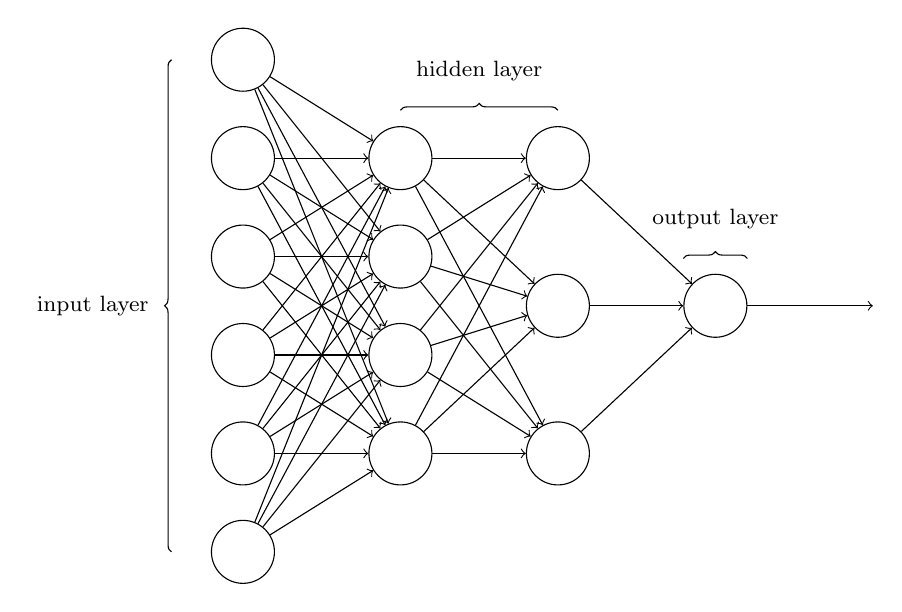
\begin{tikzpicture}[
    neuron/.style={circle,draw,inner sep=0pt,minimum size=8mm}
    ]

    % leftmost neurons:
    \foreach \y in {0,...,5}
    \node (l\y) at (0, \y * 1.25) [neuron] {};

    % left hidden layers:
    \foreach \y in {0,...,3}
    \node (hl\y) at (2, \y * 1.25 + 1 * 1.25) [neuron] {};

    % right hidden layers:
    \foreach \y in {0,...,2}
    \node (hr\y) at (4, \y * 1.875 + 1 * 1.25) [neuron] {};

    % output:
    \node (output) at (6, 3.125) [neuron] {};

    % draw brace:
    \draw[decorate,decoration={brace,mirror}] ([xshift=-5mm]l5.west) -- ([xshift=-5mm]l0.west) node [midway,xshift=-10mm] {
      \footnotesize input layer
    };

    \draw[decorate,decoration={brace}] ([yshift=2mm]hl3.north) -- ([yshift=2mm]hr2.north) node [midway,yshift=5mm] {
      \footnotesize hidden layer
    };

    \draw[decorate,decoration={brace}] ([yshift=6mm]output.west) -- ([yshift=6mm]output.east) node [midway,yshift=5mm] {
      \footnotesize output layer
    };

    % connections:
    \foreach \x in {0,...,5}
    \foreach \y in {0,...,3}
    \draw [->] (l\x) to (hl\y);

    \foreach \x in {0,...,3}
    \foreach \y in {0,...,2}
    \draw [->] (hl\x) to (hr\y);

    \foreach \y in {0,...,2}
    \draw [->] (hr\y) to (output);

    \draw [->] (output) to (8, 3.125);

  \end{tikzpicture} 
\end{document}
